% -*- root: ../AlgebraConmutativa.tex -*-
\chapter{Variedades algebraicas afines}
El objetivo de este tema es hacer geometría usando el Álgebra Conmutativa. Para ellos vamos a disponer de un 'campo de juego' y de unas 'herramientas':

\begin{center}
	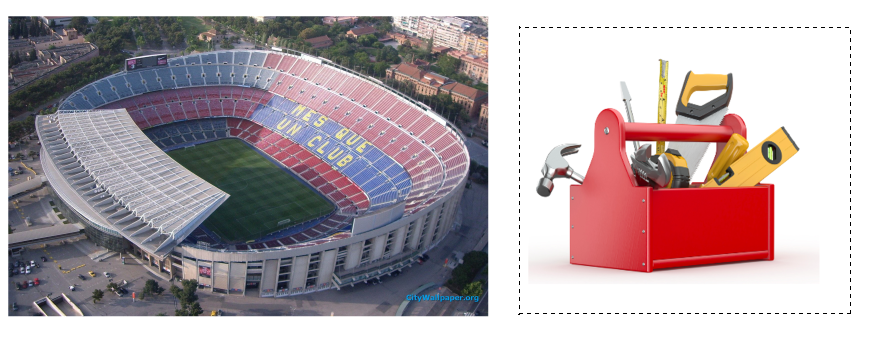
\includegraphics[scale=0.45]{img/vaa.png}
\end{center}

\begin{itemize}
	\item Nuestro 'campo de juego' no será tan increíble, exitoso y espectacular como el que aparece en la imagen. Será $\A^n_K$, o también llamado espacio afín de dimensión $n$ sobre un cuerpo $\K$ (tuplas sobre un cuerpo $\K$). Como un ejemplo vale más que x palabras con x tendiendo a 100, os pongo uno: $\A^2_{\real}$ es el plano, y las tuplas son los puntos $(x,y)$ del plano.
	\item Las herramientas serán lo que hemos dado hasta ahora, anillos noetherianos, dominios de integración, dominios de factorización única... Que empiece el juego.
\end{itemize}

\begin{defn}[Variedad algebraica]\label{def:variedad_algebraica}
	Diremos que un subconjunto $X\subset \A^n_K$ es una variedad algebraica afín si los puntos de $X$ son las únicas soluciones de alguna colección $F$ de polinomios en $\K[x_1,...,x_n]$.

	Es decir, $X$ es una variedad algebraica afín (v.a.a.) si existe $F \subset K[x_1,...,x_n]$ tal que $X=\{ (a_1,...,a_n) \in \A_K^n: p(a_1,...,a_n)=0,  \forall p(x_1,...,x_n) \in F \} = \V(F)=\text{ 'Conjunto de soluciones de F '}$.
\end{defn}

En resumen, a grandes rasgos y para entendernos tenemos que:
\begin{itemize}
	\item Dado un conjunto de ecuaciones, la variedad algebraica asociada no es más que el conjunto de puntos que son solución de esas ecuaciones.
	\item Dado un conjunto de puntos (sin obligar a que sea variedad algebraica), existirá un conjunto de polinomios que se anulen en esos puntos. Pero no se garantiza que exista un conjunto de polinomios que se anulen sólo en esos puntos.
	\item Dada una \textbf{variedad algebraica}, existe un conjunto de ecuaciones que tienen por solución únicamente los puntos pertenecientes a dicha variedad algebraica.
\end{itemize}

\obs $X$ es una variedad algebraica si y solo sí existe un sistema de ecuaciones $F$ que tiene por solución únicamente los puntos pertenecientes a X.

Vemos algunos ejemplos de variedades algebraicas afines.
\begin{example}
	\begin{itemize}
		\item $\emptyset = \V(1)$. La ecuación $1=0$ no tiene solución. $\emptyset$ siempre es una v.a.a.
		\item $\A_K^n=\V(0)$. Todos los puntos del espacio afín son solución de la ecuación $0=0$. $\A_K^n$ siempre es una v.a.a.
		\item Ahora cogemos $A^1_k$, que es la recta afín sobre un cuerpo K (por ejemplo si el cuerpo fuera $\real$, este espacio afín serían todos los puntos de $\real^1$).

		Si cojo $F=\{p(x)\}$, la variedad algebraica afín serán los puntos que son solución de la ecuación $p(x)=0$. Es decir, $\V(F)$ puede ser $\emptyset$ o un número finito de puntos, como mucho tantos como el grado de $p(x)$.
		\item Ahora vamos a coger una variedad afín y vamos a encontrar $F$. Es decir, cogemos un conjunto de puntos y buscamos qué ecuaciones son soluciones de todos a la vez.

		Por ejemplo: Sea $\K=\real$, $\{1,2,3\} =\V((x-1)(x-2)(x-3))$. Que no es lo mismo que: $\V(x-1,x-2,x-3)=\emptyset$, ya que no hay ningún valor $x$ tal que esas 3 ecuaciones sean 0 a la vez.

		De hecho la variedad algebraica anterior es más grande que lo que hemos dicho, sería: $\{1,2,3\} =\V(\gen{(x-1)(x-2)(x-3)})$. Recordemos que $\gen{(x-1)(x-2)(x-3)} = \{ p(x)(x-1)(x-2)(x-3) : p(x) \in \real[x] \}$ (todos los múltiplos de $(x-1)(x-2)(x-3)$)
	\end{itemize}
\end{example}

\obs Todo conjunto finito de puntos en $\A_K^n$ es una variedad algebraica.

\obs Sea $Y$ una colección infinita de puntos en $A^1_n$ (distinta del total), entonces $Y$ NO es una variedad algebraica afín. Ya que el conjunto de soluciones de $p(x)=0$ está acotado por el grado de $p(x)$, así que salvo que $Y=\A^n_k$, $Y$ no puede ser una v.a.a.

Así, sin mucho esfuerzo hemos descrito todas las variedades afines de la recta, que son el vacío, el total, y conjuntos finitos de puntos.

Ahora vamos a pensar en  $\A_K^2$:
\begin{example}
	Sea $\A_K^2$, entonces tenemos $K[x_1,x_2]$. Vamos a buscar $F$ para:

	\begin{enumerate}
		\item $(a_1,a_2) \in \A^2_k$.

		Probamos con $F=\{(x_1-a_1)(x_2-a_2)\}$. Que no es lo que buscamos ya que $(x_1-a_1)(x_2-a_2)=0$ tiene por solución dos rectas (las de color azul):

		\begin{center}
			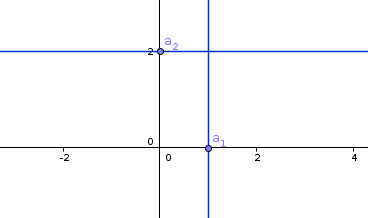
\includegraphics[scale=0.45]{img/ej1.png}
		\end{center}

		La solución buena es:  $F=\{(x_1-a_1),(x_2-a_2)\}$ ya que el sistema de ecuaciones $(x_1-a_1)=0$ y $(x_2-a_2)=0$ tiene como solución el punto de intersección de ambas rectas que es precisamente $(a_1,a_2)$.

		\begin{center}
			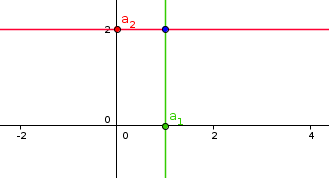
\includegraphics[scale=0.45]{img/ej2.png}
		\end{center}


		\item $(a_1,a_2),(b_1,b_2) \in \A^2_k$. Buscamos $F$

		Se nos ocurre probar con:
		\[
		\left.
		\begin{array}{rcl}
		(x_1-a_1)(x_2-b_2) & = & 0  \text{ \textcolor{green}{-----}}\\
		(x_2-a_2)(x_1-b_1) & = & 0 \text{ \textcolor{red}{-----}}
		\end{array}
		\right\}
		\]

		\begin{center}
			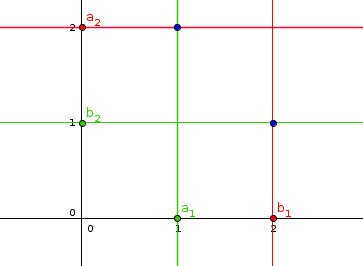
\includegraphics[scale=0.45]{img/ej3.png}
		\end{center}

		Que vale como solución salvo si $b_2=a_2$ o $a_1=b_1$ en cuyo caso nos saldría una recta como solución, que difiere de lo que buscamos que son dos puntos.

		La solución buena es:
		\[
		\left.
		\begin{array}{rcl}
		(x_1-a_1)(x_2-b_2) & = & 0 \text{ \textcolor{green}{-----}}\\
		(x_2-a_2)(x_1-b_1) & = & 0 \text{ \textcolor{red}{-----}}\\
		(x_1-a_1)(x_1-b_1) & = & 0 \text{ \textcolor{black}{-----}}\\
		(x_2-a_2)(x_2-b_2) & = & 0 \text{ \textcolor{purple}{-----}}
		\end{array}
		\right\}
		\]

		Que gráficamente es superponer el dibujo anterior con este:

		\begin{center}
			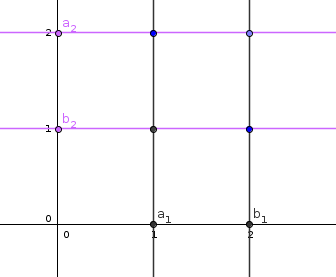
\includegraphics[scale=0.45]{img/ej4.png}
		\end{center}

		Por tanto $F=\{ (x_1-a_1)(x_2-b_2), (x_2-a_2)(x_1-b_1), (x_1-a_1)(x_1-b_1), (x_2-a_2)(x_2-b_2)  \}$
	\end{enumerate}
\end{example}


\begin{prop}
	Sea $F \subset \K[x_1,...,x_n]$ no vacío. Entonces $\V(F)=\V(\gen{F})$.
\end{prop}

\begin{proof}
	\begin{itemize}
		\item $F \subseteq \gen{F} \implies \V(F) \supset \V(\gen{F})$. Es obvio, ya que en $\gen{F}$ hay más ecuaciones que cumplir que en $F$.
		\item Vamos a ver la otra inclusión: $\V(F) \supset \V(\gen{F})$.

		Sea $(a_1,...,a_n) \in \V(F) \implies \forall p(x_1,..,x_n) \in F$, $p(a_1,...,a_n)=0$. Y para que $(a_1,...,a_n) \in \V(\gen{F})$ tenemos que ver que $\forall q(x_1,...,x_n)\in \gen{F}$, $q(a_1,...,a_n)=0$.

		Si $q(x_1,...,x_n)\in \gen{F} \implies \exists c_1(x_1,...,x_n),...,c_s(x_1,...,x_n) \in F$ y $\exists b_1(x_1,...,x_n),...,b_s(x_1,...,x_n) \in \K[x_1,..,x_n]$ tal que $q(x_1,...,x_n)=b_1c_1+...+b_sc_s$.

		Entonces $q(a_1,...,a_n)=b_1(a_1,...,a_n)c_1(a_1,...,a_n)+...+b_s(a_1,...,a_n)c_s(a_1,...,a_n) = 0$  ya que $c_i=0$.
	\end{itemize}

	Nos falta el caso de que $\V(F)=\emptyset$. Pero el $\emptyset$ está contenido en cualquier conjunto.
\end{proof}

Pero... ¿por qué es interesante que $\V(F)=\V(\gen{F})$?

Como $\gen{F}\subset \K[x_1,...,x_n] \implies \gen{F}$ es finitamente generado, es decir, existe $p_1(x_1,...,x_n),...,p_t(x_1,...,x_n)$ tal que $\gen{F} = \gen{p_1(x_1,...,x_n),...,p_t(x_1,...,x_n)} \implies \V(F)=\V(\gen{F})=\V(p_1(x_1,...,x_n),...,p_t(x_1,...,x_n))$:

\obs Toda v.a.a $X$ es igual a $\V(I)$, siendo $I$ un ideal.

\obs Toda v.a.a. es el conjunto de solución de un nº finito de ecuaciones polinómicas.

\section{Topología de Zariski en \Akn}
Sea $\Akn$, entonces tanto $\emptyset$ como $\Akn$ son v.a.a., además $\emptyset=\V(\gen{1})$ y $\Akn=\V(0)$.


\begin{itemize}
	\item Sean $X_1$ y $X_2$ dos v.a.a. $\implies$ $X_1 \cap X_2$ es v.a.a..

	Esto es cierto ya que $X_1=\V(I_1)$ y $X_2=\V(I_2)$ para $I_1,I_2$ ideales en $\K[x_1,...,x_n] \implies$
	$$X_1 \cap X_2 = \V(I_1 \cup I_2)=\V(I_1+I_2)$$

	%\textcolor{red}{$I_1$ e $I_2$ son ideales porque hemos visto que $\V(F)=\V(\gen{F})$, y $K[x_1,..,x_n]$ es noetheriano y por tanto cualquier ideal es finitamente generado}

	Conclusiones:
	\begin{enumerate}
		\item La intersección de un número finito de v.a.a. es una v.a.a.
		\item La intersección infinita de v.a.a. también es v.a.a.: Sea $\{ X_i \}_{i\in I}$ una colección de v.a.a., entonces:
		\[ \cap_{i\in I}X_i = \V(\gen{I_i, i \in I}) \]
	\end{enumerate}
	\item Sean $X_1, X_2$ dos v.a.a. $\implies X_1 \cup X_2$ es v.a.a..

	De hecho sea  $X_1=\V(I_1)$ y $X_2=\V(I_2)$,  para $I_1=\gen{f_1,...,f_s},I_2=\gen{g_1,...,g_t}$ ideales en $\K[x_1,...,x_n]$ entonces
	$$X_1 \cup X_2=\V(I_1 \cap I_2)=\V(I_1 \cdot I_2)=\gen{f_i, g_j}$$

	Conclusiones
	\begin{enumerate}
		\item La unión de un número finito de v.a.a. es una v.a.a.
		\item La unión arbitraria infinita de v.a.a. no tiene porque ser v.a.a. (Todos los enteros de $\ent$ no son v.a.a.)
	\end{enumerate}
\end{itemize}

Todo esto que hemos visto son una serie de conjeturas que son ciertas pero que aún no vamos a demostrar.

Nos quedamos con la siguiente proposición:

\begin{prop}
	Las variedades algebraicas afines satisfacen los axiomas de los cerrados de una topología. En $\Akn$ definimos la \concept{Topología\IS de Zariski}, como aquella en la que los cerrados son variedades algebraicas afines.
\end{prop}

\begin{example}
	Topología de Zanski en $\A^1_K$:
	\begin{itemize}
		\item Cerrados: $\emptyset$, $\A^1_K$ y $\{ p_1,...,p_n \} \subset \A^1_K$ (cantidad finita de puntos).
		\item Abiertos: (los complementarios de los cerrados) $\A^1_K$, $\emptyset$, y el complementario de una cantidad finita de puntos.
	\end{itemize}
\end{example}



% Clase 7/3/2016
Vamos a ver algunas propiedades de estas variedades generadas por ideales. Por ejemplo, si tomamos dos ideales $J, I ⊂ K[x_1, \dotsc, x_n]$, si $J ⊂ I$ entonces $\V(J) ⊃ \V(I)$.

Los radicales también nos darán resultados interesantes. A priori, un radical nos debería dar una variedad más pequeña al ser un ideal más grande. La cuestión es que lo que nos dará en realidad será la misma variedad.

\begin{prop} Sea $I ⊂ K[x_1, \dotsc, x_n]$ un ideal, y consideramos su radical $\sqrt{I}$. Entonces $\V(I) = \V(\sqrt{I})$.
\end{prop}

\begin{proof}

\proofpart{$⊃$}

Como $I ⊂ \sqrt{I}$, es obvio que $\V(I) ⊃ \V(\sqrt{I})$.

\proofpart{$⊂$}

Lo primero que tenemos que hacer es tener cuidado cuando el ideal es el vacío. Ahora bien, si $\V(I) = ∅$, entonces $\V(\sqrt{I}) = ∅$ igualmente, ya que hemos demostrado antes que $\V(\sqrt{I}) ⊂ \V(I)$.

Podemos suponer entonces que $\V(I) ≠ ∅$. Sea $(a_1, \dotsc, a_n) ∈ \V(I)$ o, en otras palabras, que $∀p(x_1, \dotsc, x_n) ∈ I$ se tiene que $p(a_1, \dotsc, a_n) = 0$.

Queremos demostrar que $(a_1, \dotsc, a_n) ∈ \V(\sqrt{I})$ y por lo tanto que $∀q(x_1, \dotsc, x_n) ∈ \sqrt{I}$ tengamos que $q(a_1, \dotsc, a_n) = 0$. Ahora bien, por ser $q$ elemento del radical, elevado a una potencia $m > 0$ nos dará cero, luego en particular $q(a_1, \dotsc, a_n)^m = 0$. Pero $q(a_1, \dotsc, a_n) ∈ K$ que es un cuerpo y dominio de integridad, así que si elevado a una potencia nos da $0$ tiene que ser él mismo cero, y por lo tanto $(a_1, \dotsc, a_n) ∈ \V(\sqrt{I})$.
\end{proof}

\subsection{La operación $\I(S)$}

Vamos a tomar un subconjunto $S ⊂ \A_K^n$. Nos fijaremos en todos los polinomios en $n$ variables que se anulan en $S$. Es decir, \[ \I(S) = \set{p(x_1, \dotsc, x_n) ∈ K[x_1, \dotsc, x_n] \tq ∀(a_1, \dotsc, a_n) ∈ S \; p(a_1, \dotsc, a_n) = 0} \]

No es difícil ver que $\I(S)$ es un ideal: no es vacío ($0 ∈ \I(S)$), está cerrado con la suma y la propiedad de absorción también se cumple trivialmente.

\begin{wrapfigure}{R}{0.4\textwidth}
\centering
\begin{tikzpicture}
\draw[->] (-0.5, 0) -- (3,0);
\draw[->] (0, -0.5) -- (0,2);

\draw[|-|, very thick, blue] (0,0) node[anchor = north west, yshift = -0.05cm, xshift = -0.05cm] {$0$} -- (1,0) node[below, yshift = -0.05cm] {$1$};
\end{tikzpicture}
\caption{El intervalo $[0,1]$ no es una variedad algebraica.}
\label{fig:Interv01}
\end{wrapfigure}

Ahora vamos a buscar todos los polinomios que se anulan en el intervalo $S= [0,1]$. Está claro que $\gen{y} = \I(S)$, pero no vamos a poder encontrar un conjunto de polinomios que se anules sólo en $S$. La razón es que $S = [0,1]$ no es una variedad algebraica. Esto nos va a dar un lema interesante.

\begin{lemma} Sea $S ⊂ \A_K^n$ un subconjunto del espacio afín. Entonces $\V(\I(S)) ⊃ S$, y la igualdad $\V(\I(S)) = S$ se da si y sólo si $S$ es una variedad algebraica afín.
\end{lemma}

\begin{proof} Por definición, siempre tenemos que $S ⊂ \V(\I(S))$. Supongamos que $S = \V(\I(S))$. Es claro que $S$ es una variedad algebraica afín, porque la igualdad indica que $S$ es el conjunto de ceros del ideal $\I(S)$.

Vamos a ir con la demostración al otro lado. Supongamos que $S$ es una variedad algebraica afín, y queremos demostrar que $S = \V(\I(S))$.

Como $S$ es una v.a.a., entonces $∃ J ⊂ K[x_1, \dotsc, x_n]$ tal que $S = \V(J)$, luego $J ⊂ \I(S)$. Entonces podemos hacer una cadena \[ S = \V(J) ⊃ \V(\I(S)) ⊃ S \], por lo que todas las inclusiones tienen que ser igualdades.
\end{proof}

Este lema lo podemos relacionar con la topología de Zariski que veíamos antes, que nos decía que los cerrados eran las variedades algebraicas.

\begin{corol} Sea $S ⊂ \A_K^n$. Entonces la \concept{Clausura\IS de Zariski} de $S$ es $\adh{S} = \V(\I(S))$, y entonces $\adh{S}$ es la variedad algebraica más pequeña que contiene a $S$.
\end{corol}

\begin{proof}
Sabemos que $S ⊂ \V(\I(S))$, donde $\V(\I(S))$ es una variedad algebraica afín. Tenemos que probar que además es la variedad más pequeña que contiene a $S$.

Hacemos la demostración por reducción al absurdo, suponiendo que existe una variedad algebraica afín $X ⊃ S$ y además $X \subsetneq \V(\I(S))$. Ahora bien, es obvio que $\I(S) ⊃ \I(X) ⊃ \I(\V(\I(S)))$. Podemos volver a tomar la variedad y entonces \[ \V(\I(S)) ⊂ \underbracket{\V(\I(X))}_{ = X} ⊂ \underbracket{\V(\I(\V(\I(S))))}_{= \V(\I(S)))} \], luego $X = \V(\I(S))$, contradicción.
\end{proof}

Dos observaciones:

\begin{prop}
Dado $S ⊂ \A_K^n$, el ideal $\I(S)$ es un ideal radical.
\end{prop}

\begin{proof} Ejercicio para el lector.
\end{proof}


Continuemos hablando sobre $\I(S)$. Sean los espacios $\Akn$ y $\K[x_1,...,x_n]$. Sea un conjunto de puntos $X \in \Akn$ ($X$ puede ser v.a.a o no), entonces existen muchos ideales $J \in \K[x_1,...,x_n]$ tales que los puntos de $X$ anulan los polinomios de $J$.

Sin embargo:

\begin{defn}
	Sea S un subconjunto de puntos, llamamos $\I(S)$ al ideal más grande formado por los polinomios que se anulan en $S$.
\end{defn}

\begin{example}
	Sea $\K=\real$ y sea $\real[x,y]$. Entonces tenemos que $S=\{(a_1,a_2)\}=\V(\gen{x-a_1,y-a_2})=\V(\gen{(x-a_1)^2+(y-a_2)^2})$. Es decir, tenemos varios conjuntos $F_i$ tal que $\V(F_i)=S$.

	Sin embargo, $\I(S)=\gen{x-a_1,y-a_2}$.
\end{example}

\begin{defn}[Ideal\IS de definición]
	Sea X una variedad algebraica afín, llamamos ideal de definición de $X$ a $\I(X)$.
\end{defn}


Si hemos entendido lo que llevamos hasta ahora, deberíamos entender el siguiente razonamiento:

Vamos a hacer el siguiente camino: primero cogemos un conjunto de puntos $S$ y obtenemos el conjunto de polinomios que se anulan en $S$(o sistema de ecuaciones que tienen por solución los puntos de $S$, que es lo mismo), es decir, $\I(S)$. Pues en general, si cogemos ahora la variedad algebraica afín $\V(\I(S))$, es decir, los puntos que se anulan en el conjunto de polinomios $\I(S)$, lo que va a ocurrir es que $\V(\I(S))$ sea más grande que $S$. Y solo serán iguales si $S$ es una variedad algebraica afín.


\begin{example}
	Tomamos el ejemplo que teníamos antes. Sea $S=[0,1] \subset \A_k^2$ con $\K=\real$.

	\begin{wrapfigure}{R}{0.4\textwidth}
		\centering
		\begin{tikzpicture}
		\draw[->] (-0.5, 0) -- (3,0);
		\draw[->] (0, -0.5) -- (0,2);

		\draw[|-|, very thick, blue] (0,0) node[anchor = north west, yshift = -0.05cm, xshift = -0.05cm] {$0$} -- (1,0) node[below, yshift = -0.05cm] {$1$};
		\end{tikzpicture}
	\end{wrapfigure}

		Queremos calcular $\V(\I(S))$. Nuestra conjetura es que la clausura de Zariski de S es $\cls{S}=\V(\I(S))=\V(\gen{y})$. Queremos probar que $\I(S)=\gen{y}$. Claramente $\gen{y} \subset \I(S)$, ya que cualquier polinomio múltiplo de $y$ se anula en los puntos  de $S$. Vamos a probar el otro contenido:

		$\gen{y} \supset \I(S)$) Sea $p(x,y) \in \I(S)$, lo expresamos de la siguiente manera: $p(x,y)=yq(x,y)+r(x)$. Por hipótesis $\forall\{a_1,a_2\} \in S$, tenemos que $p(a_1,a_2)=0$. Si $a_1$, $a_2 \in S$, entonces $a_1 \in [0,1]$ y $a_2=0$ $\implies p(a_1,a_2)=p(a_1,0)=0$.

		Y si sustituimos en nuestra expresión: $p(a_1,0)=0\cdot q(a_1,0)+r(a_1)=0 \implies r(a_1)=0 \; \forall a_1 \in [0,1] \implies r(x)=0$.

		Por tanto nos queda $p(x,y)=yq(x,y) \implies p(x,y) \in \gen{y}$.
\end{example}

\obs Sean $X$ y $X_1$ v.a.a.: Si $X_1 \subset X \implies \I(X) \subset \I(X_1)$

\begin{defn}[Variedad algebraica afín\IS irreducible] \label{def:VaaIrreducible}
	Diremos que una v.a.a. $X \subset \A^n_K$ es irreducible $\Leftrightarrow$ cada vez que escribimos $X=X_1 \cup X_2$ con $X_1, X_2$ v.a.a., se tiene que $X=X_1$ o $X=X_2$.
\end{defn}

\begin{example}
	\begin{itemize}
	\item Un punto en $\A_K^n$ es siempre irreducible.
	\item En $\A^2_{\real}$, $\V(\gen{xy})=\V(\gen{x}) \cup \V(\gen{y})$, por tanto no es irreducible.
	\item En $\A^2_{\K}$ $X=\V(\gen{y^2-x})$ es irreducible. También lo es $X=\V(\gen{y^2-x^3})$ y $X=\V(ax+by+c)$. Estudiaremos formas de ver cuándo una v.a.a. es irreducible o no.
	\end{itemize}
\end{example}

\begin{prop} \label{prop:VaaIrreducibleIdPrimo}
	Sea $X \subset \A_K^n$ una v.a.a., entonces $X$ es irreducible $\Leftrightarrow$ $\I(X)$ es primo.
\end{prop}

\begin{proof}

	\proofpart{$\implies$}

	Supongamos que $X$ es irreducible, entonces tenemos que probar que $\I(X)$ es primo. Suponemos que no. Entonces $\exists p(x_1,...,x_n), q(x_1,...,x_n) \notin \I(X)$ pero que $p\cdot q \in \I(X)$.

	Sea $J_1=\I(X)+\gen{p(x_1,...,x_n)}$ (recordemos que la notación '+' quiere decir que es el ideal más pequeño que contiene a ambos ideales.) y $J_2=\I(X)+\gen{q(x_1,...,x_n)}$. Entonces $\I(X) \subsetneqq J_1$ y $\I(X) \subsetneqq J_2$.

	Como $p(x_1,...,x_n) \notin \I(X)$, hay puntos de $X$ donde $p(x_1,...,x_n) \neq 0 \implies X \not\subset \V(p(x_1,...,x_n)) \implies \V(J_1)=\V(\I(X)) \cap \V(p(x_1,...,x_n)) \subsetneqq X$. Que por ser $X$ una v.a.a. nos quedaría  $\V(J_1) = X \cap \V(p(x_1,...,x_n)) \subsetneqq X$

	Por la misma razón $\V(J_2)=X\cap \V(q(x_1,...,x_n)) \subsetneqq X$

	Por tanto, afirmamos que: $X=\V(J_1)\cup \V(J_2)=\V(J_1 \cdot J_2)=\V(\underbrace{\I(X)^2}_{\in \I(X)}+\underbrace{\I(X)\gen{ p(x_1,...,x_n)}}_{\in \I(X)}+\underbrace{\I(X)\gen{q(x_1,...,x_n)}}_{\in \I(X)}+\underbrace{\gen{q(x_1,...,x_n)}\gen{p(x_1,...,x_n)}}_{\in \I(X) \text{ por hipotesis}}) = \V(\I(X))=X$

	Lo que es una contradicción porque $X$ es irreducible.

	\proofpart{$\impliedby$}

	Supongamos que $\I(X)$ es primo entonces queremos probar que entonces $X$ es irreducible.

	Supongamos que $X$ no es irreducible $\implies \exists X_1,X_2 \subset \A_K^n$ v.a.a. tal que $X=X_1 \cup X_2$ pero $X_1 \subsetneqq X$ y $X_2 \subsetneqq X$ $\implies \I(X) \subsetneqq \I(X_1)$ y $\I(X) \subsetneqq \I(X_2)$ $\implies$ $\exists p_1(x_1,...,x_n) \in \I(X_1) \setminus \I(X)$ y $\exists p_2(x_1,...,x_n) \in \I(X_2)\setminus \I(X)$.

	Vamos a probar que: $p_1(x_1,...,x_n)p_2(x_1,...,x_n) \in \I(X)$ para llegar a contradicción. Es decir, vamos a probar que si $\{a_1,...,a_n\} \in X$, entonces $p_1(a_1,...,a_n)p_2(a_1,...,a_n)=0$.

	Si $\{a_1,...,a_n\} \in X = X_1 \cup X_2 \implies \underbrace{\{a_1,...,a_n\}\in X_1}_{p_1(a_1,...,a_n)=0}$ ó $\underbrace{\{a_1,...,a_n\}\in X_2}_{p_2(a_1,...,a_n)=0}$

	Luego hemos encontrado dos polinomios $p_1$ y $p_2$ que no están en $\I(X)$ pero su producto si está en $\I(X) \implies \I(X)$ no es primo $\implies$ contradicción con la hipótesis inicial.
\end{proof}

\begin{example}
	Antes hemos dicho que, en $\A^2_{\K}$, $X=\V(\gen{y^2-x})$ es irreducible. Vamos para ello a ver que $\I(X)$ sea primo.

	Sabemos que $\gen{y^2-x} \subset \I(X)$ \textcolor{red}{Por que? por que es el ideal as grande? Entonces en el ejemplo anterior podríamos haber usado el mismo argumento en vez de decir que se anulan los puntos en S y tal}. Supongamos que el contenido es estricto, es decir que $\gen{y^2-x} \subsetneqq \I(X)$.

	Para ello nos ayudamos del paso al cociente, sabemos que $\I(X) \subset \real[x,y]$. Entonces nos queda \[ \real[y] \simeq \quot{\real[x,y]}{\gen{y^2-x}} \supset \quot{\I(X)}{\gen{y^2-x}}  \neq \{\cls{0}\} \], donde $\quot{\I(X)}{\gen{y^2-x}}$ ha de ser no nulo porque si lo fuera implicaría que $\I(X) = \gen{y^2 -x}$ (todos los polinomios de $\I(X)$ serían múltiplos de $y^2 - x$). Así, existe un polinomio no nulo $p(y) ∈ \quot{\I(X)}{\gen{y^2-x}}$, que sólo depende de la variable $y$ por la relación de equivalencia $\cls{x} = y^2$.

	Por tanto, tendríamos que tanto $\gen{y^2-x}$ como $\gen{p(y)}$ están contenidos en $\I(X)$. Ahora miramos a $\V(\I(X)) \subset \underbrace{\V(\gen{y^2-x}) \cap \V(p(y))}_{\text{nº finito de puntos}}$.

	\begin{wrapfigure}{R}{0.35\textwidth}
		\centering
		\vspace{-15pt}
		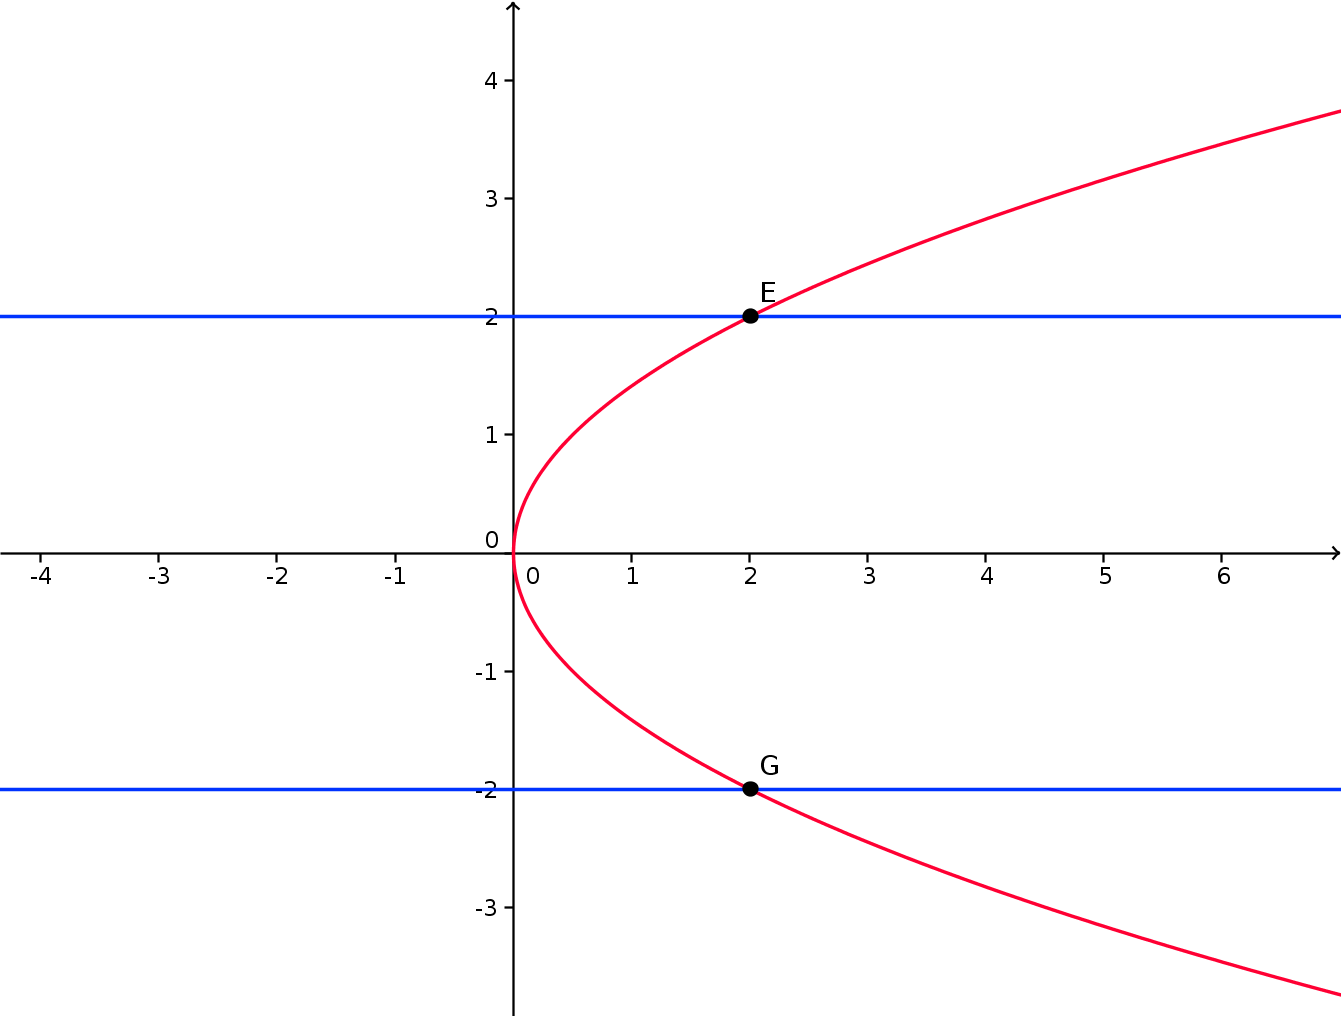
\includegraphics[width=0.32\textwidth]{img/parabola.png}
		\caption{Los puntos de la intersección son siempre una cantidad finita.}
		\label{fig:ParabolaRectas}
	\end{wrapfigure}

	Es un número finitos porque primero fijamos los puntos que anulan los polinomios de la forma $\gen{y^2-x}=p(x,y)\cdot(y^2-x)$, que son infinitos puntos de una parábola.

	Después nos fijamos en los que anulan los polinomios $\gen{p(y)}$, que también son infinitos. De hecho, serán rectas de la forma $y = c$ ya que el polinomio no depende de $x$. Por ejemplo, si $p(y)=y^2-4$, serán dos rectas $y=2$ e $y=-2$. La cuestión es que cada $p(y)$ se anula en un número finito de rectas (si no sería el polinomio nulo). Por tanto, la intersección entre ambos conjuntos será finita. Con este ejemplo serían solo dos puntos, como en la \fref{fig:ParabolaRectas}.

	Por tanto llegamos a una contradicción y $\I(X)=\gen{y^2-x}$, es un ideal primo y por lo tanto $X$ es irreducible. \noteby{Guille}{No veo muy clara la contradicción.}
\end{example}

\begin{theorem}
	Toda v.a.a. $X$ en $\Akn$ se puede escribir como una unión finita de v.a.a. irreducibles y salvo el orden y si evitamos redundancias, esa escritura es única.
\end{theorem}

\begin{proof}
	Supongamos que existe al menos una v.a.a. en $\Akn$ que no se puede escribir como una unión de una cantidad finita de v.a.a. irreducibles.

	Sea $\Sigma=\{ X \subseteq \Akn: X \text{ no es unión de v.a.a. irreducibles }\}$. $\Sigma \neq \emptyset$ por hipótesis.

	Sea $\hat{\Sigma}=\{\I(X): X \in \Sigma\}$. Luego $\hat{\Sigma} \neq \emptyset$. Como estamos en $\Akn$ y $\K$ es noetheriano, entonces $\K[x_1,...,x_n]$ también es noetheriano, y el conjunto $\hat{\Sigma}$ tiene un elemento maximal $J=\I(Y)$ con $Y \in \Sigma$ (Ver proposición \ref{prop:caracterizacion_noetheriano}). Entonces $Y=\V(\I(Y))$ es un elemento \textbf{minimal} en $\Sigma$.

	Como $Y \in \Sigma \implies Y$ no es irreducible $\implies Y_1,Y_2$ v.a.a. $\subset \Akn$ tal que $Y=Y_1 \cup Y_2$ y además $Y_1,Y_2 \subsetneqq Y \underbrace{\implies}_{\text{ Y minimal }} Y_1, Y_2 \notin \Sigma \implies  Y_1$ e $Y_2$ se pueden escribir como unión finita de irreducibles $\implies$ $Y$ también es unión finita de irreducibles en contradicción con la hipótesis.

	\textbf{Unicidad:} Supongamos que $X=X_1\cup...\cup X_s=Y_1 \cup...\cup Y_t$ con $X_i \not \subset X_j$,  $i \neq j$ $Y_l \not \subset Y_m$, $l \neq m$ (para evitar redundancia),  y $X_i$ e $Y_l$ irreducibles $\forall i=1,...,s$, $\forall l=1,...,t$.

	Cogemos:
	$$ \underbrace{X\cap Y_1}_{=Y_1}=(X_1 \cup X_2 \cup ... \cup X_n) \cap Y_1 = (X_1 \cap Y_1) \cup (X_2 \cap Y_2) \cup ... \cup (X_s \cap Y_1)$$

	Como $Y_1$ es irreducible, $\exists j$ tal que $Y_1=X_j \cap Y_1 \implies Y_1 \subset X_j$.

	Cogemos ahora:
	$$ \underbrace{X \cap X_j}_{= X_j} = (Y_1 \cup Y_2 \cup ... \cup Y_t) \cap X_j = (Y_1 \cap X_j) \cup (Y_2 \cap X_j) \cup ... \cup (Y_t \cap X_j)$$

	Como $X_j$ es irreducible, $\exists i$ tal que $X_j=Y_i \cap X_j \implies X_j \subset Y_i$

	Por tanto nos queda:

	$Y_1 \subset X_j \subset Y_i \implies Y_1 \subset Y_i \implies i=1 \implies Y_1 = X_j$

	Se concluye mediante un argumento inductivo.
\end{proof}

